\section{Results}
\label{sec:results}

\subsection{Exp~1: the discriminator separates the regimes cleanly}
\label{sec:results_exp1}

\Tabref{tab:exp1_main} reports accuracy by condition and \tabref{tab:discriminator} the
discriminator metrics; \figref{fig:exp1} visualizes both. Three patterns emerge, one per
regime.

\begin{table}[t]
    \centering
    \resizebox{\textwidth}{!}{%
    \begin{tabular}{@{}llccccc@{}}
        \toprule
        \textbf{Model} & \textbf{Setting} & \textbf{Regime} & \textbf{no-skill} & \textbf{correct} & \textbf{self-gen} & \textbf{length-ctrl} \\
        \midrule
        \multirow{5}{*}{\claude}
          & \arithbten   & elicitation      & 0.983 & 0.967 & 0.983 & 0.950 \\
          & \vocabes     & elicitation      & 0.950 & \textbf{1.000} & \textbf{1.000} & 0.950 \\
          & \arithbnine  & novelty-proc     & 0.850 & 0.883 & \textbf{0.250} & 0.850 \\
          & \arithbeleven& novelty-proc     & 0.767 & 0.683 & 0.767 & 0.750 \\
          & \vocabzeth   & novelty-info     & \textbf{0.000} & \textbf{1.000} & \textbf{0.000} & \textbf{0.000} \\
        \midrule
        \multirow{5}{*}{\gpt}
          & \arithbten   & elicitation      & 0.417 & \textbf{0.700} & 0.367 & 0.250 \\
          & \vocabes     & elicitation      & 0.917 & \textbf{1.000} & 0.850 & 0.917 \\
          & \arithbnine  & novelty-proc     & 0.000 & 0.000 & 0.000 & 0.000 \\
          & \arithbeleven& novelty-proc     & 0.017 & 0.000 & 0.000 & 0.017 \\
          & \vocabzeth   & novelty-info     & \textbf{0.000} & \textbf{1.000} & \textbf{0.000} & \textbf{0.000} \\
        \bottomrule
    \end{tabular}
    }
    \caption{\textbf{Exp~1: accuracy by condition} ($N=60$ held-out items; bootstrap 95\% CIs in
    the text). The decisive row is \vocabzeth on both models: the correct skill lifts accuracy
    $0.00\to1.00$ while the self-generated skill and length-matched control stay at $0.00$ ---
    genuine, un-self-generatable new knowledge. In the elicitation settings a length-matched
    irrelevant memo matches the ``skill.'' The self-generated \arithbnine skill \emph{hurts}
    \claude ($0.85\to0.25$). Bold marks the informative contrasts.}
    \label{tab:exp1_main}
\end{table}


\para{Novelty-information: genuine, un-self-generatable knowledge.} On \vocabzeth both models
move from $0.00$ with no skill to $1.00$ with the correct skill, while the self-generated skill
and the length-matched control both stay pinned at $0.00$. This gives the maximal \END
signature: normalized gain $g_{\text{correct}}=1.00$, self-generation utility $\SG=0.00$,
length-controlled gain $\LCG=1.00$, two-proportion $p<10^{-4}$, and Cohen's $h=3.14$ (the
theoretical maximum for a $0\to1$ shift). The correct skill is decisive, the self-generated
skill and the irrelevant memo are worthless, and the knowledge is provably absent from the base
model. This is the one unambiguous ``new knowledge'' case in the study.

\para{Elicitation: the skill is prompt-shaping, not teaching.} On \vocabes and \arithbten the
model can write its own working skill ($\SG\approx1$ for Spanish on \claude), and a
length-matched irrelevant memo does about as well as the ``skill'' (Spanish: $0.95$ vs $0.95$).
The lone execution-limited exception is \gpt on base-10 multiplication, where the correct skill
helps $0.42\to0.70$ ($p=0.002$): a scaffolding effect on a procedure that is still fully latent,
not an injection of new knowledge.

\para{Novelty-procedure: a capability floor.} On \arithbnine and \arithbeleven the correct skill
barely helps \claude (execution, not knowledge, is the bottleneck), and \gpt fails at $\sim0$
regardless of skill --- an in-context skill cannot buy compute the model lacks. Most striking,
\claude's \emph{self-generated} base-9 skill actively \emph{hurts}, dropping accuracy from
$0.85$ to $0.25$: it articulated a harder, more error-prone algorithm than its own default. A
self-generated skill is a sampled elicitation strategy, and a worse one can interfere.

\begin{figure}[t]
    \centering
    \begin{subfigure}[b]{0.48\textwidth}
        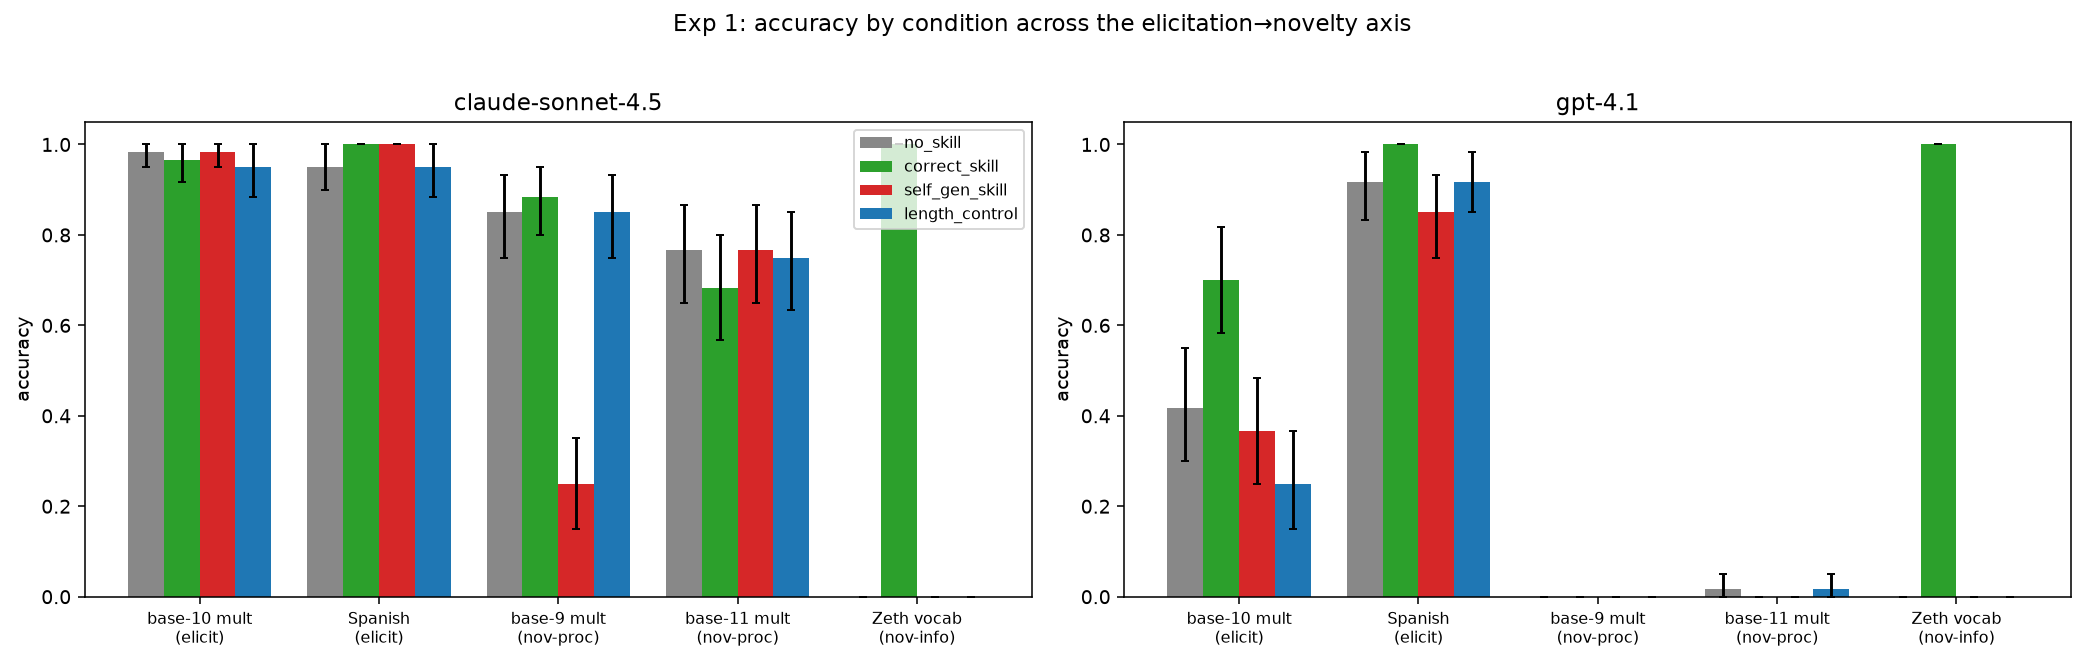
\includegraphics[width=\textwidth]{figures/exp1_condition_bars.png}
        \caption{Accuracy by condition}
        \label{fig:exp1_bars}
    \end{subfigure}
    \hfill
    \begin{subfigure}[b]{0.48\textwidth}
        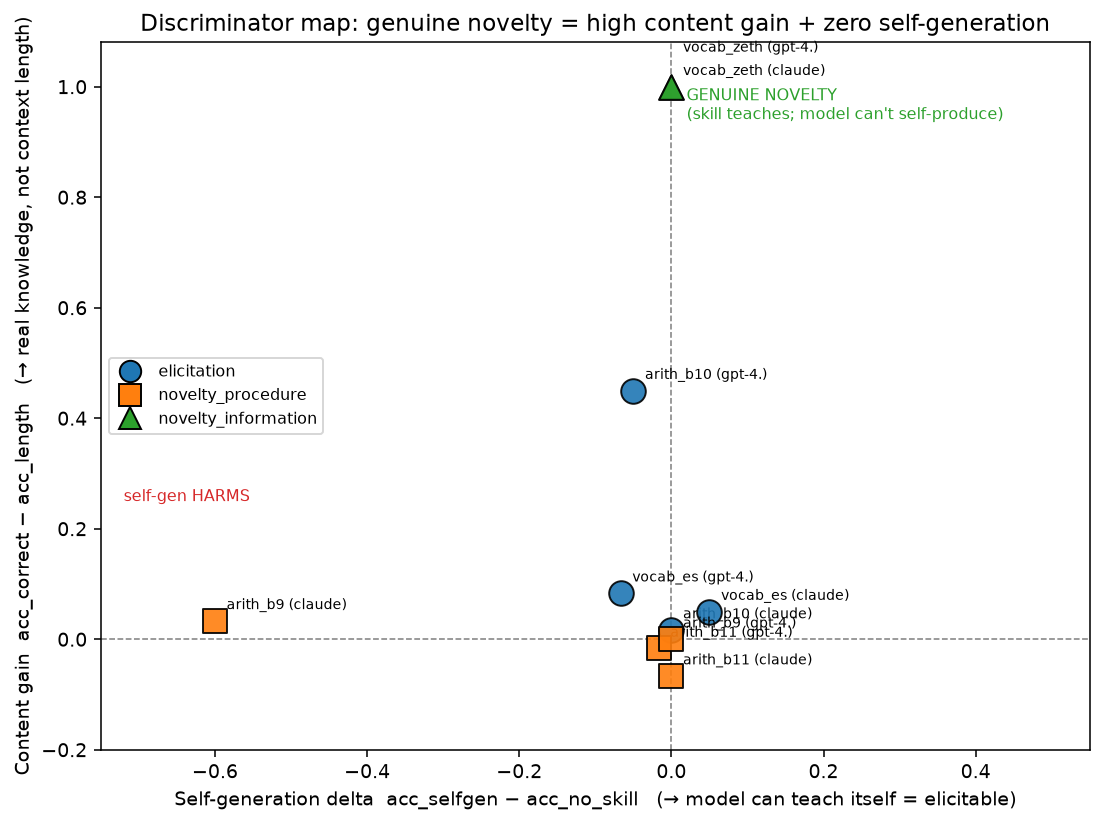
\includegraphics[width=\textwidth]{figures/exp1_discriminator_scatter.png}
        \caption{Discriminator scatter (\SG vs \LCG)}
        \label{fig:exp1_scatter}
    \end{subfigure}
    \caption{\textbf{Exp~1.} \captiona\ Accuracy across the four conditions and five settings:
    only \vocabzeth shows a large correct-skill gain that neither self-generation nor the length
    control can reproduce. \captionb\ In the discriminator plane, novelty-information sits at
    low \SG / high \LCG (genuine new knowledge), while elicitation settings sit at high \SG with
    a length control that matches the skill.}
    \label{fig:exp1}
\end{figure}

\begin{table}[t]
    \centering
    \resizebox{\textwidth}{!}{%
    \begin{tabular}{@{}llcccccc@{}}
        \toprule
        \textbf{Model} & \textbf{Setting (regime)} & $g_{\text{correct}}$ & \textbf{\SG} & \textbf{\LCG} & $p_{\text{corr vs base}}$ & \textbf{Cohen's }$h$ \\
        \midrule
        \claude & \vocabzeth (novelty-info)   & \textbf{1.00} & \textbf{0.00} & \textbf{1.00} & $<10^{-4}$ & \textbf{3.14} \\
        \gpt    & \vocabzeth (novelty-info)   & \textbf{1.00} & \textbf{0.00} & \textbf{1.00} & $<10^{-4}$ & \textbf{3.14} \\
        \midrule
        \claude & \vocabes (elicitation)      & 1.00 & 1.00 & 1.00 & 0.079 & 0.45 \\
        \claude & \arithbten (elicitation)    & --   & --   & --   & 0.559 & $-0.11$ \\
        \gpt    & \arithbten (elicitation)    & 0.49 & $-0.18$ & 0.77 & 0.002 & 0.58 \\
        \midrule
        \claude & \arithbnine (novelty-proc)  & 0.22 & $-18.0$ & 0.22 & 0.591 & 0.10 \\
        \claude & \arithbeleven (novelty-proc)& $-0.36$ & $-0.0$ & $-0.29$ & 0.307 & $-0.19$ \\
        \bottomrule
    \end{tabular}
    }
    \caption{\textbf{Exp~1: discriminator metrics.} The novelty-information setting (\vocabzeth)
    shows the maximal signature on both models: decisive gain ($g=1.00$), zero self-generation
    utility ($\SG=0.00$), positive length-controlled gain ($\LCG=1.00$), and maximal effect size
    ($h=3.14$). Elicitation settings show $\SG\approx1$ and a length control that matches the
    skill. For \arithbten on \claude, $g$ is undefined/unstable at ceiling (baseline $0.983$), so
    we read that row from absolute accuracies. The self-generated \arithbnine skill has strongly
    negative \SG because it actively lowers accuracy.}
    \label{tab:discriminator}
\end{table}


\subsection{Exp~2: self-evolution is bounded by latency plus external signal}
\label{sec:results_exp2}

\Tabref{tab:exp2} and \figref{fig:exp2} show the self-evolution learning curves. The decisive
contrast is \vocabzeth: verifier-only self-evolution stays at $0.00$ for all five iterations,
because pass/fail feedback leaks essentially no information about 24 arbitrary word mappings, so
introspection cannot manufacture them. The instant the loop receives ground-truth answers it
climbs to $0.85$, copying the revealed mappings into a glossary. This is exactly the
AlphaEvolve~\citep{alphaevolve} and cannot-self-correct~\citep{cannotselfcorrect} pattern: an
external, non-gameable signal is what turns self-evolution into discovery. For the \emph{latent}
base-9 procedure, self-evolution recovers even from verifier-only feedback (up to $0.95$),
because the knowledge was already there to elicit; and the elicitation setting \vocabes stays
flat near ceiling under both signals.

\begin{table}[t]
    \centering
    \resizebox{\textwidth}{!}{%
    \begin{tabular}{@{}llccc@{}}
        \toprule
        \textbf{Setting} & \textbf{knowledge} & \textbf{verifier-only (iter 1$\to$5)} & \textbf{with-answer (iter 1$\to$5)} & \textbf{correct-skill ceiling} \\
        \midrule
        \arithbnine (novelty-proc) & latent   & $0.28 \to 0.08 \to 0.90 \to 0.95 \to \mathbf{0.93}$ & $0.38 \to 0.95 \to \cdots \to \mathbf{0.95}$ & 0.875 \\
        \vocabzeth (novelty-info)  & absent   & $0.00 \to 0.00 \to 0.00 \to 0.00 \to \mathbf{0.00}$ & $\mathbf{0.85}$ (from iter 1, stable) & 1.000 \\
        \vocabes (elicitation)     & latent   & $\sim0.87$ (flat)                                   & $\sim0.90$ (flat, near ceiling)          & 1.000 \\
        \bottomrule
    \end{tabular}
    }
    \caption{\textbf{Exp~2: self-evolution learning curves} (\claude, $K=5$, disjoint 40-item
    test set). Verifier-only self-evolution never moves \vocabzeth off $0.00$ across all five
    iterations --- pass/fail leaks essentially no information about 24 arbitrary word mappings
    --- but with-answer feedback reaches $0.85$ immediately. For the \emph{latent} base-9
    procedure, verifier-only self-evolution recovers on its own, because it is eliciting
    knowledge already present.}
    \label{tab:exp2}
\end{table}


\begin{figure}[t]
    \centering
    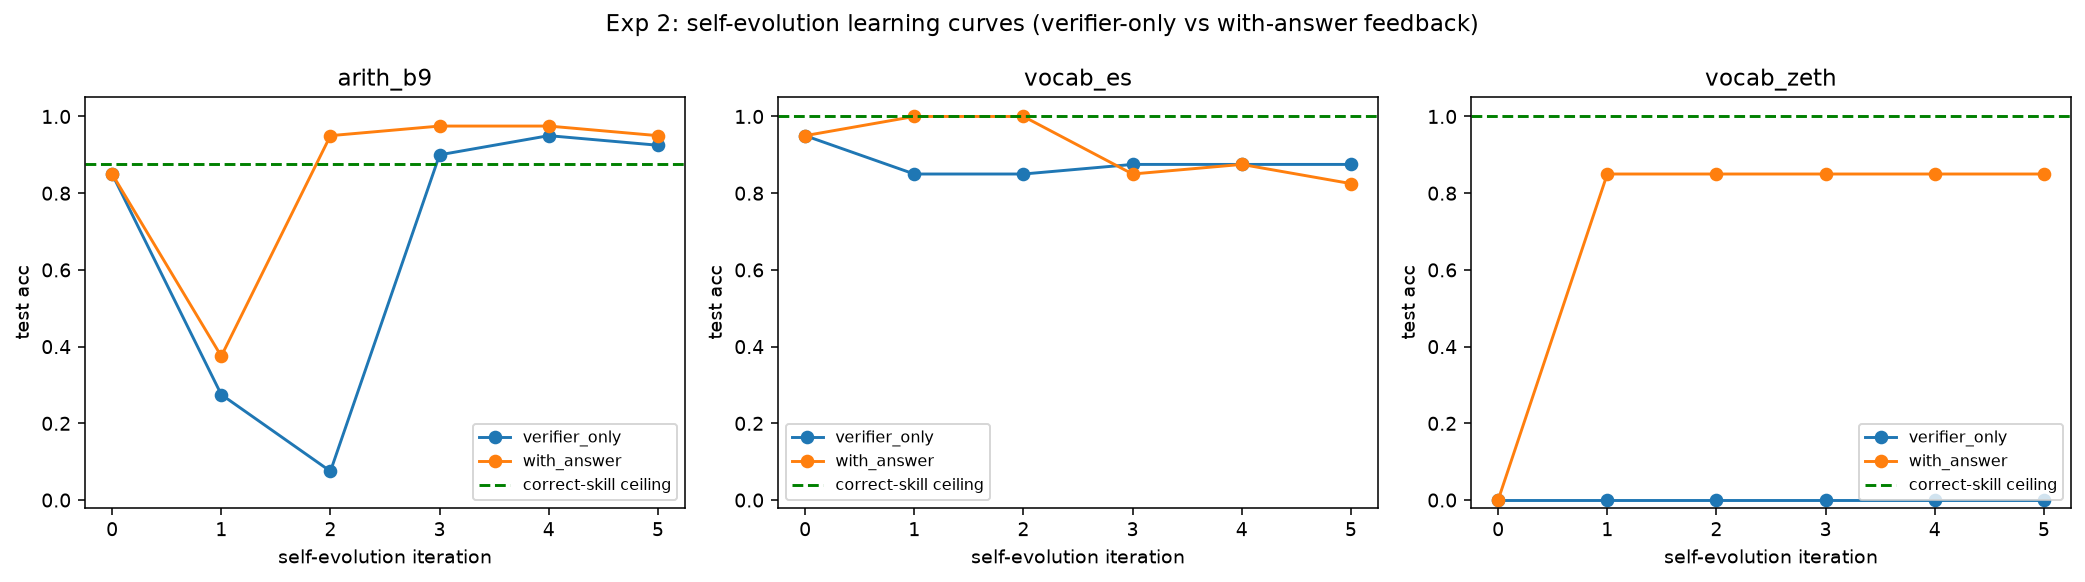
\includegraphics[width=0.72\linewidth]{figures/exp2_self_evolution.png}
    \caption{\textbf{Exp~2: self-evolution learning curves} (\claude, $K=5$). Under
    verifier-only feedback (pass/fail) \vocabzeth never leaves $0.00$, while the latent base-9
    procedure recovers on its own. With-answer feedback unlocks \vocabzeth immediately. Genuine
    novelty enters the loop only through the external ground-truth signal.}
    \label{fig:exp2}
\end{figure}

\subsection{Exp~3: the ``fine-tune it back'' probe is real but method-dependent}
\label{sec:results_exp3}

\Tabref{tab:exp3} and \figref{fig:exp3} report the internalization probe. For \zeth,
example-distillation writes the glossary into the weights so \qwen translates \emph{held-out}
phrases at $1.00$ with nothing in context --- proof that the skill encoded real, transferable
knowledge rather than a prompt trick. But fine-tuning on the \emph{document} (the same
information, as prose) internalizes nothing ($0.00$). The user's proposed probe therefore
cannot by itself classify a skill: its verdict flips with the fine-tuning recipe, and a naive
document-finetune would wrongly declare real, transferable knowledge to be mere prompt
optimization. For base-9 multiplication the 7B model fails at $0.00$ in every condition ---
an in-context skill and light fine-tuning alike cannot supply executional capacity it lacks.

\begin{table}[t]
    \centering
    \resizebox{0.85\textwidth}{!}{%
    \begin{tabular}{@{}lcccc@{}}
        \toprule
        \textbf{Setting} & \textbf{base (no skill)} & \textbf{in-context skill} & \textbf{LoRA on \emph{document}} & \textbf{LoRA on \emph{examples}} \\
        \midrule
        \vocabzeth (novelty-info)  & 0.00 & 0.95 & \textbf{0.00} & \textbf{1.00} \\
        \arithbnine (novelty-proc) & 0.00 & 0.00 & 0.00 & 0.00 \\
        \bottomrule
    \end{tabular}
    }
    \caption{\textbf{Exp~3: internalization probe} (\qwen, held-out test, \emph{no} skill in the
    prompt unless labelled in-context). For \zeth, example-distillation writes the glossary into
    the weights so the model translates held-out phrases at $1.00$ with nothing in context ---
    proof of real, transferable knowledge --- but fine-tuning on the \emph{document} internalizes
    nothing ($0.00$). The ``fine-tune it back'' probe therefore cannot by itself classify a
    skill: its verdict flips with the recipe. Base-9 fails at $0.00$ in every condition (a
    capability floor a 7B model cannot cross).}
    \label{tab:exp3}
\end{table}


\begin{figure}[t]
    \centering
    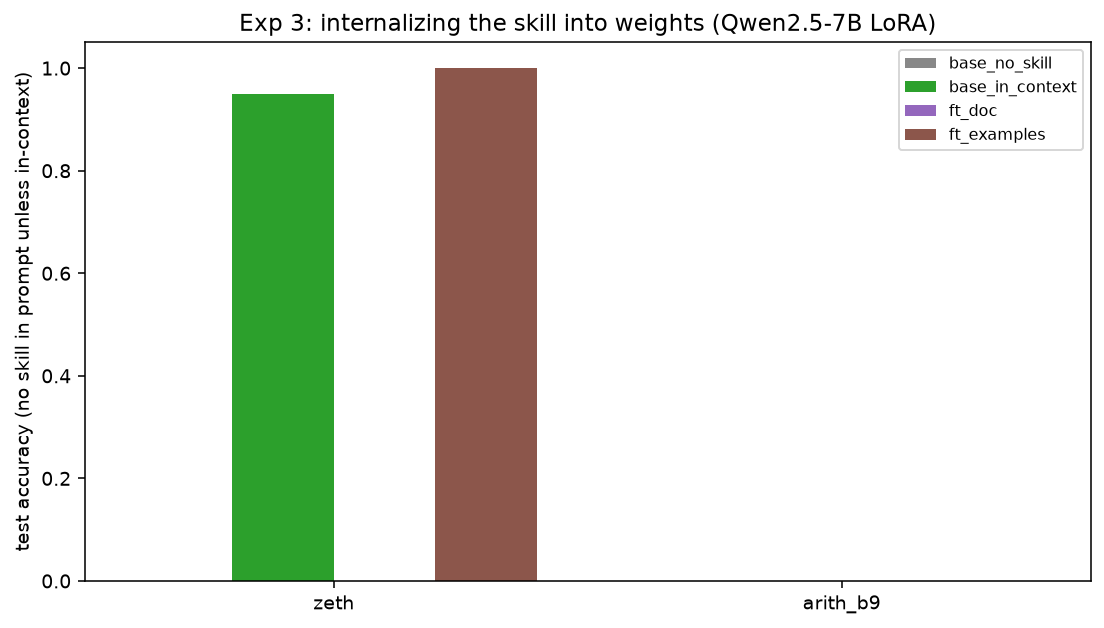
\includegraphics[width=0.72\linewidth]{figures/exp3_internalization.png}
    \caption{\textbf{Exp~3: internalization probe} (\qwen, no skill in context unless labelled).
    Example-distillation internalizes the \zeth glossary and generalizes to held-out phrases
    ($1.00$); document fine-tuning internalizes nothing ($0.00$). The fine-tune-back probe is
    recipe-dependent and cannot alone distinguish novelty from elicitation.}
    \label{fig:exp3}
\end{figure}
